\documentclass[a4paper, 12pt]{amsart}
\usepackage[french]{babel}
\usepackage[utf8]{inputenc}
\usepackage{amssymb}
\usepackage{graphicx}
\usepackage{coursebook}
\fthmstyle{plain}
\newfancythm{fthm}{Théorème}
\fthmstyle{defn}
\newfancythm{fdefn}{Définition}
\fthmstyle{ex}
\newfancythm{fex}{Exercice}
%\DeclareMathOperator*{\ln}{ln}
\newcommand{\pd}[2]{\ensuremath{\frac{\partial #1}{\partial #2}}}
\usepackage{pgf,tikz}
\usetikzlibrary{arrows, shapes}
\usetikzlibrary[patterns]
\usetikzlibrary{calc,fadings,decorations.pathreplacing, bending} 
\usetikzlibrary{decorations.markings}
\usetikzlibrary{decorations.pathmorphing}
\usetikzlibrary{positioning}
\usetikzlibrary{intersections}
\usetikzlibrary{hobby}

\title{Questions de cours et exercices pour l'examen final}

\begin{document}
\maketitle
\section{Questions de cours}
Les questions proposées dans ce document portent sur le cours et sont regroupées en thèmes. Lors de l'examen final, seules les questions de cette liste pouront être
posées, avec un minium de une dans chaque thème.
\subsection{Thème holomorphie}
Dans cette partie, le terme domaine d'holomorphie désigne le plus grand ouvert
dans lequel une application est holomorphe.
\begin{enumerate}
\item Quel est le domaine d'holomorphie de $f : z \mapsto z^4$ ?
\item Quel est le domaine d'holomorphie de $f : z \mapsto |z|$ ?
\item)Quel est le domaine d'holomorphie de $f : z \mapsto 1/ \cos(z)$ ?
\item Quel est le domaine d'holomorphie de $f : z \mapsto 1/(1 + z^2 )$ ?
\item Quel est le domaine d'holomorphie de $f : z \mapsto e^z /(1 + z^2 )$ ?
\item L'application $z \mapsto z\overline{z}$ est-elle holomorphe en $z = 1$ ?
\item Expliquer pourquoi l'application $z \mapsto z^2$ est holomorphe dans $\C$ et donner
sa dérivée.
\item Si $f, g$ sont deux applications holomorphes dans $\C$ , l'application $f.g$ est-elle
holomorphe ? Quelle est sa dérivée ?
\item Si $f, g$ sont deux applications holomorphes dans $\C$ , l'application composée
$f \circ g$ est-elle holomorphe ? Quelle est sa dérivée ?
\item Si $f, g$ sont deux applications holomorphes dans $\C$, en quels points l'appli-
cation $f /g$ est-elle holomorphe ? Quelle est sa dérivée ?
\end{enumerate}
\subsection{Thème séries entières et fonctions analytiques}
\begin{enumerate}
\item Enoncer le critère de d'Alembert pour une série de terme général $a_n$.
\item A l'intérieur de son disque ouvert de convergence, une application définie
par une série entière est-elle holomorphe ? Si oui, comment exprime-t-on sa
dérivée ?
\item Quel est le rayon de convergence de la série $\sum_{n \geq 0} x^n / n!$ ?
\item Quel est le rayon de convergence de la série $\sum_{n \geq 0} (-1)^n x^n / n!$ ?
\item
\item Énoncer le théorème des zéros isolés.
\end{enumerate}
\subsection{Thème formule de Cauchy}
\begin{enumerate}
	\item Soit $\gamma$ le lacet $t \in [0, 2\pi] \mapsto e^{it}$ . Que vaut :
	\[
	\int_\gamma \frac{dz}{z} \quad ?
	\] 
	\item Soit $\gamma$ le lacet $t \in [0, 2\pi] \mapsto e^{it}$ . Que vaut :
	\[
	\int_\gamma \frac{\sin z}{z} dz \quad ?
	\] 
	\item Soit $\gamma$ un lacet simple de classe $C^1$ . Soit $f$ une application holomorphe dans
	$\C$ . Que vaut :
		\[
	\int_\gamma f(z) dz \quad ?
	\] 
	\item Soit  $\gamma$  un lacet simple de classe $C^1$ ne passant pas par $z_0 \in \C$ . Soit $f$ une
	application holomorphe dans C . Que vaut :
	\[
\int_\gamma \frac{f(z)}{z-z_0} dz \quad ?
\] 
		\item Soit  $\gamma$  un lacet simple de classe $C^1$ ne passant pas par $z_0 \in \C$ . Soit $f$ une
	application holomorphe dans C . Que vaut :
	\[
	\int_\gamma \frac{f(z)}{(z-z_0)^2} dz \quad ?
	\] 
\end{enumerate}
\subsection{Thème série de Laurent et résidus}
\begin{enumerate}
	\item Donner le développement en série de Laurent de $z \mapsto e^z$ au voisinage de 0.
	\item Donner le développement en série de Laurent de $z \mapsto 1+z+z^{-1}$ au voisinage de 0.
	\item Enoncer le théorème des résidus.
	\item Quel est le résidu en 0 de l'application $z \mapsto cos(z)/z$ ?
	\item Quel est le résidu en $i$ de l'application $z \mapsto 1/(1 + z^2 )$ ?
	\item Soit $\gamma$ le lacet $t \in [0, 2\pi] \mapsto 2e^{it}$ . Que vaut :
\[
\int_{\gamma} \frac{e^z}{1+z^2}dz\quad ?
\]
	\item Soit $\gamma$ le lacet $t \in [0, 2\pi] \mapsto 2e^{it}$ . Que vaut :
	\[
	\int_{\gamma} \frac{z}{1+z}dz\quad ?
	\]
\end{enumerate}
\section{Exercices vus en cours}
Si $f$ est une application intégrable telle que:
\[
\int_\R \left | f(t) \right| dt < +\infty
\]
sa transformée de Fourier est l'application $\widehat{f}$ définie par:
\[
\widehat{f} \colon \omega \in \R \mapsto \int_{\R} f(t) \exp(-i \omega t ) dt
\]
\begin{fex}
    On dit qu'une application $\phi \colon \C \to \C$ est une isométrie si, pour tout couple
    de complexes $(z_0,z_1)$, on a $\lvert \phi(z_1)-\phi(z_0)\rvert = \lvert z_1-z_0\rvert.$ 
    Soit $C$ un compact de $\C$ et $\phi$ une isométrie telle que $\phi(C) \subset C.$
    \begin{itemize}
        \item Montrer que $\phi$ est continue et injective.
        \item On suppose que $C-\phi(C) \neq \emptyset.$ Soit $u \in C -\phi(C).$ Montrer qu'il existe un réel non nul $\delta$ et un point $z_0 \in \phi(C)$ tels que:
        \[
        \delta = \inf_{z \in \phi(C)} \lvert u - z \rvert = \lvert u - z_0 \rvert.
        \]
        \item Montrer qu'il existe une sous-suite de la suite $\phi^n(u), n \geq 1$ convergeant 
        vers $u$.
        \item En déduire que $\phi$ est surjective, donc bijective.
    \end{itemize}
\end{fex}
\begin{itemize}
    \item Par définition d'une isométrie, $\phi$ est lipschitzienne, donc continue. Par ailleurs, si $\phi(z_1)=\phi(z_0)$, alors $\lvert \phi(z_1) - \phi(z_0)\rvert = \lvert z_1 - z_0 \rvert = 0$, prouvant que $\phi$ est injective.
    \item $\phi(C)$ est compact comme image d'un compact par une application continue. L'application:
    \[
        z \in \phi(C) \mapsto \lvert u- z \rvert 
    \]
    est continue, donc atteint ses bornes, d'où la propriété demandée.
    \item $\phi(C)$ étant compact, il existe une sous-suite convergente, notée $\phi^{n_i}(u), i \in \N$, de la suite $\phi^{n}(u), n \geq 1$. $\phi$ étant une isométrie, on a:
    \[
    \lvert \phi^{n_{i+1}}(u) - \phi^{n_i}(u)  \rvert = \lvert \phi^{n_{i+1}-n_i}(u) - u \rvert
    \]
    d'où l'existence d'une sous-suite de la suite $\phi^{n}(u), n \geq 1$ convergeant vers $u$.
    \item S'il existe une suite de $\phi(C)$ convergeant vers $u$, alors $\delta=0$, ce qui est une contradiction. On en déduit $\phi(C)=C$ et donc la surjectivité de $\phi.$ Comme $\phi$ est injective, elle est bijective.
\end{itemize}


\begin{fex}
   Montrer que $\C$ et $\R$ ne sont pas homéomorphes. 
    
    \textbf{Indication:} Montrer que si $\phi \colon \C \to \R$ est un homéomorphisme, alors $\Phi\left(\C-\{0\}\right)$ n'est pas connexe.    
\end{fex}
Si $\phi$ est un homéomorphisme, il n'existe pas de complexe $z$ tel que $\phi(z)=\phi(0)$ et donc
$\phi\left(\C - \{0\}\right)=\R-\{\phi(0)\}.$ Ce sous-ensemble de $\R$ est un ouvert qui n'est pas
connexe par arc, alors que $\C - \{0\}$ l'est, ce qui est contradictoire.

\begin{fex}
 Soit $\Omega$ un domaine non vide de $\mathbb{C}$ et soit $f$ application
holomorphe sur $\Omega$. Montrer que les conditions suivantes sont
équivalentes~:
\renewcommand{\theenumi}{\alph{enumi}}
\begin{enumerate}
\item $f$ est constante sur $\Omega$.
\item $\Re(f)$ est constante sur $\Omega$.
\item $\Im(f)$ est constante sur $\Omega$.
\item $|f|$ est constante sur $\Omega$.
\end{enumerate}
\end{fex}
On séparera partie réelle et partie imaginaire de $f$ en posant $f=P+iQ$
Il est clair que (a) implique les autres conditions. Si on suppose (b), par
application des conditions de Cauchy et en utilisant que $P$ est constant:
\[
 \pd{P}{x} = \pd{Q}{y} = 0 , \pd{P}{y}=-\pd{Q}{x} = 0
\]
$\Omega$ étant connexe, on en déduit $Q$ constante. Il s'agit en fait d'une
équivalence $(b) \Leftrightarrow (c)$, le même raisonnement s'appliquant à $Q$.
On montre donc en sus que $|f|^2=P^2+Q^2$ est aussi une constante.
Finalement, si l'on suppose $P^2+Q^2$ constant, les dérivées partielles de
cette application par rapport à $x,y$ donnent;
\[
 P\pd{P}{x}+Q\pd{Q}{x}= 0,\,  P\pd{P}{y}+Q\pd{Q}{y}= 0
\]
En utilisant les conditions de Cauchy:
\[
 P\pd{P}{x}-Q\pd{P}{y}= 0,\,  P\pd{P}{y}+Q\pd{P}{x}= 0
\]
Il s'agit d'un système linéaire homogène de déterminant $P^2+Q^2=|f|^2$. Si
cette quantité est nulle, alors $f$ est nulle et (a) est vérifiée. Sinon:
\[
 \pd{P}{x}=\pd{P}{y}=0
\]
prouvant que $P$ est une constante et donc aussi $Q$ car $(b) \Leftrightarrow
(c)$, soit $f$ constante.

\begin{fex}
Soit $\Omega$ un ouvert de $\C$ ne contenant pas $0.$ Soit $f=P + i Q \colon \Omega \to \C$ une application $\R$ dérivable. Montrer, en posant $z=re^{i\theta}$ pour $z \in \Omega$, que les conditions de Cauchy en un point $z_0 = r_0 e^{i \theta_0}$ sont équivalentes à:
\[
\begin{cases}
    \frac{\partial P}{\partial r}\vert_{r_0,\theta_0} = \frac{1}{r}\frac{\partial Q}{\partial \theta}\vert_{r_0,\theta_0} \\
    \frac{\partial P}{\partial \theta}\vert_{r_0,\theta_0} =- r\frac{\partial Q}{\partial r}\vert_{r_0,\theta_0}
\end{cases}
\]
\end{fex}
Il s'agit d'une application de la dérivation en chaîne. En posant $z = x + i y$, $f = P + i Q$ 
et en supposant vérifiées les conditions de Cauchy en coordonnées cartésiennes:
\begin{equation}
\begin{split}
    & \frac{\partial P}{\partial r} = \frac{\partial P}{\partial x}\frac{\partial x}{\partial r} +\frac{\partial P}{\partial y}\frac{\partial y}{\partial r}
    = \frac{\partial Q}{\partial y} \cos \theta -\frac{\partial Q}{\partial x} \sin \theta\\
    & \frac{\partial Q}{\partial \theta} = \frac{\partial Q}{\partial x}\frac{\partial x}{\partial \theta} + \frac{\partial Q}{\partial y}\frac{\partial y}{\partial \theta} = -\frac{\partial Q}{\partial x} r \sin\theta + \frac{\partial Q}{\partial y} r \cos \theta
\end{split}
\end{equation}
Par identification:
\[
\frac{\partial P}{\partial r} = \frac{1}{r}\frac{\partial Q}{\partial \theta}
\]
De même:
\begin{equation}
\begin{split}
    & \frac{\partial P}{\partial \theta} = \frac{\partial P}{\partial x}\frac{\partial x}{\partial \theta} +\frac{\partial P}{\partial y}\frac{\partial y}{\partial \theta}
    = - \frac{\partial Q}{\partial y} r \sin \theta -\frac{\partial Q}{\partial x} r \cos \theta\\
    & \frac{\partial Q}{\partial r} = \frac{\partial Q}{\partial x}\frac{\partial x}{\partial r} + \frac{\partial Q}{\partial y}\frac{\partial y}{\partial r} = \frac{\partial Q}{\partial x}  \cos \theta + \frac{\partial Q}{\partial y} \sin \theta
\end{split}
\end{equation}
d'où:
\[
\frac{\partial P}{\partial \theta} = -r \frac{\partial Q}{\partial r}
\]
\begin{fex}
    Soit $\Omega$ un ouvert de $\C$ contenant l'origine et $f \colon \Omega \to \C$ une application développable en
    série entière au voisinage de $0$, de rayon de convergence $r > 0$. On dira que $z_0 \in \Omega$ est un point singulier de $f$ si $f$ n'est développable en série entière dans aucune boule ouverte de centre $z_0$ et de rayon non nul.
    \begin{itemize}
        \item Montrer qu'il ne peut exister aucun point singulier dans la boule ouverte $B(0,R).$
        \item Montrer qu'il existe au moins un point singulier sur $\partial B(0,R) = \Bar{B}(0,R)-B(0,R).$
    \end{itemize}
    On admettra la propriété suivante, qui est démontrée dans le chapitre sur les séries de Laurent: Une application holomorphe dans un domaine $\Omega$ est développable en série entière dans tout disque ouvert contenu dans $\Omega.$
\end{fex}
Cet exercice montre que le rayon de convergence est égal à la distance au plus proche point singulier. 
Si $z_0$ appartient à $D(0,R)$, alors il existe $\eta > 0$ tel que $D(z_0,\eta) \subset D(0,R).$ Soit $z \in D(z_0,\eta)$, alors:
\begin{equation}
\label{eq:sum_z_z0}
\begin{split}
f(z) & = \sum_{n\in \N} a_n z^n = \sum_{n \in \N} a_n \left(
z-z_0 + z_0
\right)^n \\
& = \sum_{n\in \N} a_n z^n = \sum_{n \in \N} a_n \sum_{k=0}^n
\frac{n!}{k!(n-k)!} \left( z-z_0 \right)^k z_0^{n-k}
\end{split}
\end{equation}
Cette série est absolument convergente car:
\[
\lvert z-z_0 \rvert ^k \lvert z_0 \rvert^{n-k} \leq \eta^k \lvert z_0 \rvert^{n-k}
\]
d'où:
\[
\begin{split}
\sum_{n \in \N} \lvert  a_n \rvert \sum_{k=0}^n
\frac{n!}{k!(n-k)!} \lvert z-z_0 \rvert^k \lvert z_0\rvert ^{n-k} 
& \leq \sum_{n \in \N} \lvert  a_n \rvert \sum_{k=0}^n
\frac{n!}{k!(n-k)!} \eta^k \lvert z_0 \rvert^{n-k}\\
& \leq \sum_{n \in \N} \lvert  a_n \rvert \left( \eta + \lvert z_0 \rvert \right)^n < +\infty
\end{split}
\]
Il est donc possible d'intervertir les sommes dans \ref{eq:sum_z_z0} ce qui donne:
\begin{equation}
\begin{split}
 f(z) & = \sum_{n\in \N} a_n z^n = \sum_{n \in \N} \left(z-z_0\right)^n \sum_{k \geq n} a_k \frac{k!}{n! (k-n)!}z_0^{k-n} \\ 
  & = \sum_{n \in \N} \frac{f^{(n)}(z_0)}{n!} \left(z-z_0\right)^n
  \end{split}
\end{equation}
On a donc démontré la proposition suivante: en tout point $z_0$ du disque ouvert de convergence, l'application $f$ est égale à son développement en série de Taylor dans un disque $D(z_0,\eta).$

Pour la seconde question, supposons qu'il n'existe pas de point singulier sur le cercle $\mathcal{C}(0,r)=\partial B(0,r).$ Il est alors possible de recouvrir $\mathcal{C}(0,r)$ par des boules ouvertes non vides sur lesquelles $f$ est développable en série entière:
\[
\mathcal{C}(0,r) \subset \cup_{z \in \mathcal{C}(0,r)} B(z,r_z), \, r_z > 0
\]
Comme $\mathcal{C}(0,r)$ est compact, il existe un nombre fini de telles boules vérifiant:
\[
\mathcal{C}(0,r) \subset \cup_{i=1}^n B(z_i, r_i), z_i \in \mathcal{C}(0,r), \, r_i > 0, \, i=1\dots n.
\]
On en déduit que l'application $f$ se prolonge en une application analytique dans un disque ouvert $B\left(0,r+\eta\right),\, \eta > 0$ et admettra donc un développement en $0$ de rayon de convergence strictement plus grand que $r$, ce qui est une contradiction.
\begin{fex}
Montrer que le développement en serie entière de 
\[\frac{e^z}{1+z}\]
a pour terme général:
\[a_n=(-1)^n \left[\frac{1}{2!} - \frac{1}{3!} + \cdots + \frac{(-1)^n}{n!}\right], \quad n \geq 2.\]

Quel est le rayon de convergence de la série ?
\end{fex}
On utilise la formule du produit de Cauchy qui donne directement le terme général $a_n.$

Le rayon de convergence est $1$ par application du critère de d'Alembert.
\begin{fex}
 Soit la série entière:
\[
f \colon z \mapsto \sum_{n >0}(-1)^{n-1}\frac{(z-1)^n}{n}
\]
\begin{enumerate}
  \item Déterminer son rayon de convergence;
  \item Montrer que pour tout réel $x \in ]0,2[$, $f(x)=\log(x)$;
  \item En déduire que $f$ est l'unique application analytique prolongeant le
  logarithme réel sur le disque ouvert $B(1,1)$;
  \item Vérifier que sur $B(1,1)$, on a $\exp \circ f = Id$.
\end{enumerate}
\end{fex}
\begin{enumerate}
 \item On utilise le critère de d'Alembert. Le rapport de deux termes
consécutifs est $n/(n+1)$, de limite 1 à l'infini. Le rayon de convergence est
donc 1.
\item Résultat classique de classes préparatoires. On peut dériver terme à
terme la série dans son disque ouvert de convergence, qui donne la série:
\[
\sum_{n >0}(-1)^{n} (z-1)^n = \frac{1}{1+(z-1)}
\]
La valeur particulière $f(1)=0$ permet alors de conclure.
\item $f$ coïncide avec $\log$ sur une partie possèdant un point d'accumulation
(en fait, tout le segment réel $]0,2[$). Par le principe du prolongement
analytique, elle est unique.
\item Toujours sur le segment $]0,2[$, $\exp \circ f = \exp \circ \log = Id$.
Par prolongement analytique de l'application $\exp \circ f$, cette égalité est
vraie sur $B(1,1)$.
\end{enumerate}
% \begin{fex} %\label{ex:int_1surz}
% Soit la fonction :
% \[f(z)= \frac{1}{z}
% \]
% Calculer son intégrale sur le cercle unité $ \{ z \in \C \, | \, \| z \| = 1 \}$ que l'on pourra par exemple paramétrer par
% \begin{align*}
%     \gamma \colon [0;1] & \to \C \\
%                      t  & \mapsto e^{2 \pi i t}
% \end{align*}
% Plus généralement, calculer l'intégrale de $f$ sur $\gamma_R = \{ z \in \C \, | \, \| z \| = R \}$ avec $R > 0$. Que remarque-t-on ?
% Enfin, calculer l'intégrale de $f$ sur le contour $- \gamma : t \in [0;1] \mapsto e^{-2 \pi i t}$
% \end{fex}
\begin{fex}
 Soit l'application $f \colon z \mapsto \exp\left(i z^2\right)$. 
\begin{enumerate}
  \item Montrer que $f$ est holomorphe sur $\mathbb{C}$ et vérifier que sa
  dérivée est continue.
  \item Pour tout réel $r > 0$, le contour $\gamma_r$ est défini selon la figure
  \ref{fig:contour2}. Donner la valeur de l'intégrale:
  \[
  \int_{\gamma_r} f(z) dz
  \]
  \item Ecrire cette intégrale sous la forme d'une somme de trois
  intégrales de chemin et montrer que l'intégrale correspondant à l'arc de
  cercle tend vers 0 lorsque $r \to +\infty$.
  \item En déduire les valeurs des intégrales généralisées suivantes, dites
  intégrales de Fresnel:
  \[
  \lim_{r \to +\infty} \int_{[-r,r]} \cos(x^2) dx, \quad  \lim_{r \to +\infty}
  \int_{[-r,r]} \sin(x^2) dx
  \]
\end{enumerate}
\end{fex}
 \begin{figure}[ht]
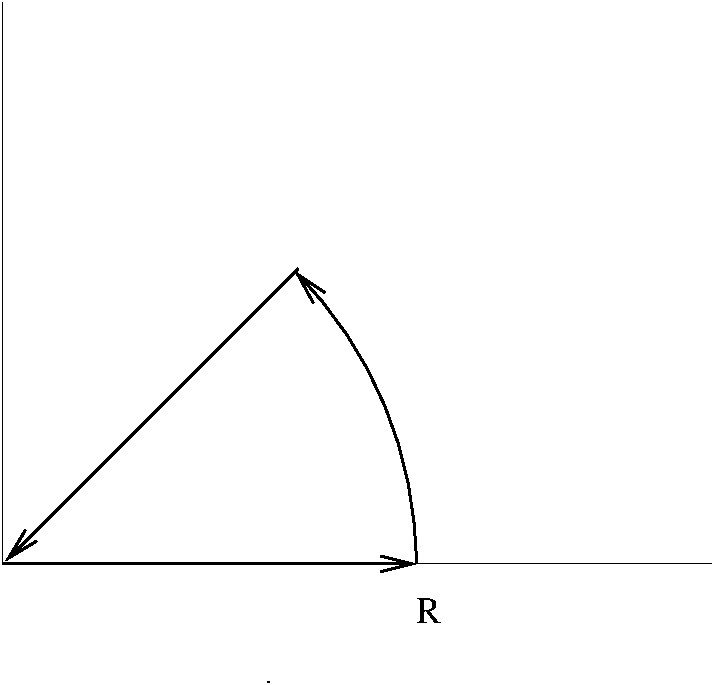
\includegraphics[scale=0.3]{images/contour_fresnel.pdf}
\caption{Contour $\gamma_r$}\label{fig:contour2}
\end{figure}
\begin{enumerate}
\item L'application $f$ est holomorphe comme composée d'applications
holomorphes. Sa dérivée est $f^\prime(z) = 2 i z f(z)$, qui est continue. 
\item
Par la formule de Cauchy, on a~:
\[
\int_{\gamma_3 . \gamma_2 . \gamma_1} f(z) dz = 0
\]
Par ailleurs~:
\[
\int_{[0,R]} e^{ix^2}d \lambda(x) = \int_{\gamma_1} f(z) dz
\]
En choisissant pour $\gamma_2$ le paramètrage~:
\[
t \in [0, \frac{\pi}{4}] \to \gamma_2(t) = R e^{it}
\]
on obtient~:
\[
\int_{\gamma_2} f(z) dz = \int_{[0, \frac{\pi}{4}]} e^{-R^2 \sin (2t)
+ i R^2 \cos(2t)} i R e^{it} d \lambda(t)
\]
On peut majorer le module de $\int_{\gamma_2} f(z) dz$ par~:
\[
\int_{[0, \frac{\pi}{4}]} e^{-R^2 \sin (2t)}  R d \lambda(t)
\]
Comme l'application $\sin$ est concave sur $[0, \frac{\pi}{2}]$, sur
cet intervalle on a~: $\sin(t) \geq \frac{2 t}{\pi}$, ce qui donne la
majoration~:
\[
\left | \int_{\gamma_2} f(z) dz \right | \leq 
\int_{[0, \frac{\pi}{4}]} e^{-\frac{R^2 4 t}{\pi}} R dt =
\frac{(\pi)(1- e^{-R^2})}{4 R}
\]
\item
\[
\int_{\gamma_3} f(z) dz = e^{i \frac{\pi}{4}} \int_{[0,R]} e^{-t^2} d\lambda(t)
\]
d'où en passant à la limite et en remarquant que $\lim_{R \to
+\infty}\int_{\gamma_2} f(z) dz = 0$~:
\[
I = J = \frac{1}{2} \sqrt{\frac{\pi}{2}}
\]
\end{enumerate}
\begin{fex}
 Soit $f \colon z \in \mathbb{C} \mapsto \exp(-z^2)$.
\begin{enumerate}
  \item Montrer que $f$ est holomorphe dans $\mathbb{C}$, de dérivée continue.
  \item En utilisant le contour $\gamma_r$ donné figure \ref{fig:contour3},
déterminer, pour
  $\omega \in \mathbb{R}$ fixé, la valeur de l'intégrale:
  \[
  \int_{\gamma_r} \exp(-z^2)dz
  \]
  \item En faisant tendre $r$ vers $+\infty$ et en faisant un raisonnement
  similaire à celui de l'exercice précédent, déterminer la transformée de
  Fourier de l'application $x \mapsto \exp(-x^2)$.
\end{enumerate}
\end{fex}
 \begin{figure}[ht]
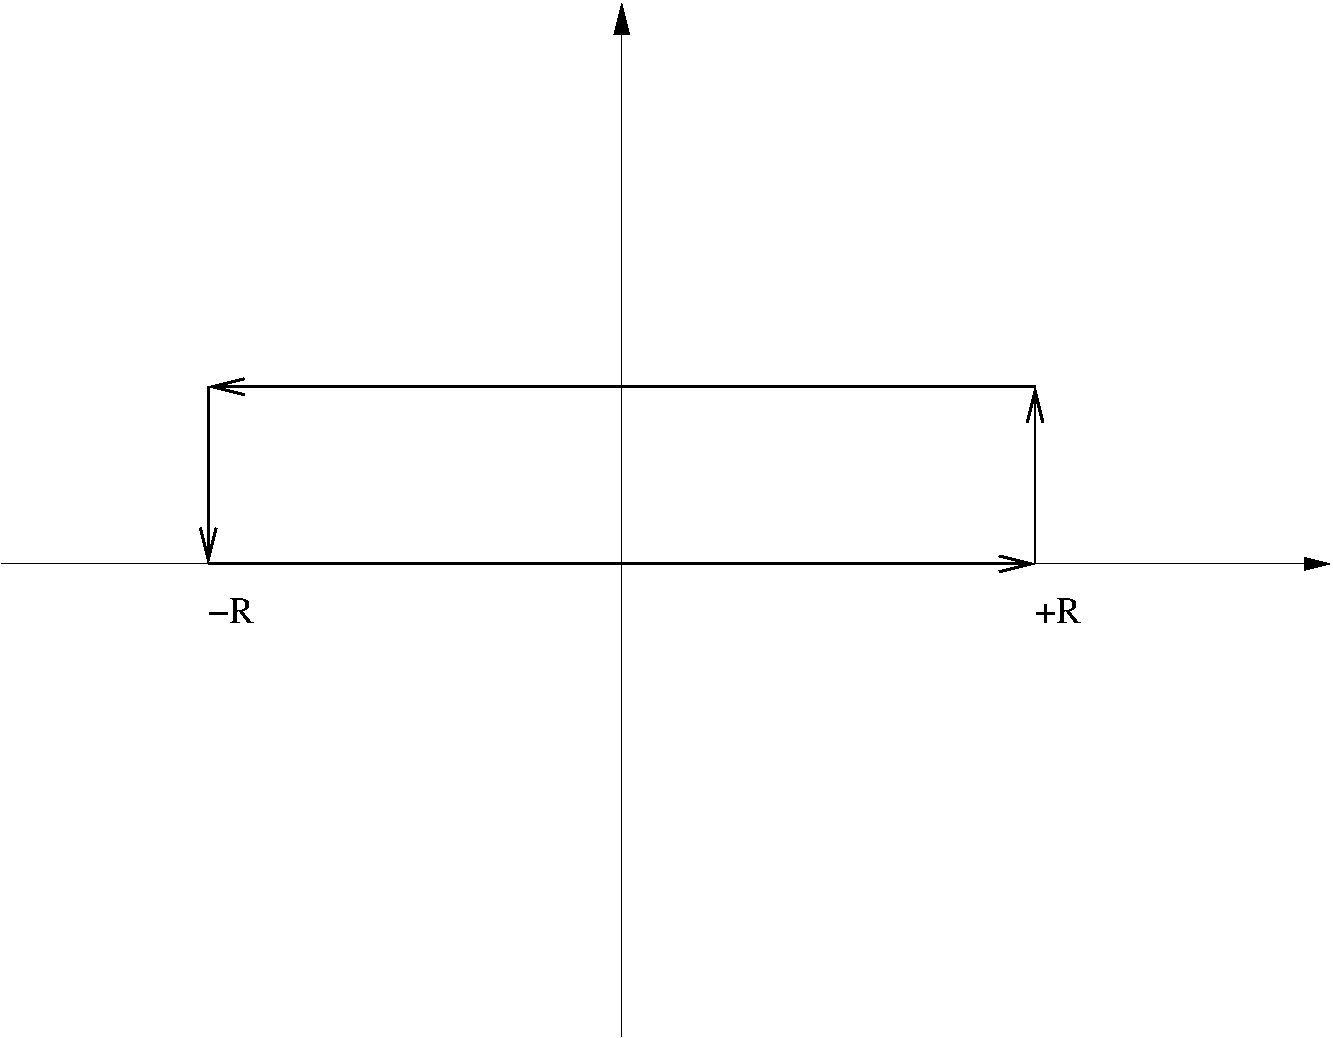
\includegraphics[scale=0.3]{images/contour_gauss.pdf}
\caption{Contour $\gamma_r$}\label{fig:contour3}
\end{figure}
\begin{enumerate}
 \item Même raisonnement que dans l'exercice précédent.
\item L'application intégrée est holomorphe, la formule de Cauchy s'applique:
\[
  \int_{\gamma_r} \exp(-z^2)dz = 0
  \]
\item L'intégrale sur l'axe réel est:
\[
 \int_{[-r,r]} \exp(-x^2) dx 
\]
de limite $\sqrt{\pi}$ pour $r \to +\infty$. Le segment supérieur se paramètre
par:
\[
 t \in [-r,r] \mapsto -t+i \frac{\omega}{2}
\]
L'intégrale le long de ce chemin est donc:
\[
 - \int_{[-r,r]} e^{-t^2 + i t \omega + \frac{\omega^2}{4}} dt
\]
La limite lorsque $r\to +\infty$ est:
\[
- e^{\frac{\omega^2}{4}} \int_\R  e^{-t^2 + i t \omega} dt 
\]

Finalement, l'intégrale sur les segments verticaux aura pour limite $0$ si $r
\to +\infty$. Un paramétrage possible du segment situé en $r$ est:
\[
t \in [0, \frac{\omega}{2}] \mapsto r + it 
\]
conduisant à l'intégrale:
\[
 i \int_{[0, \frac{\omega}{2}]} e^{-(r+it)^2} dt 
\]
son module se majore par:
\[
 \frac{\omega}{2}e^{-r^2 + \frac{\omega^2}{4}}
\]
qui a bien pour limite $0$ lorsque $r \to +\infty$. Le second segment vertical
se traite de la même façon. En regroupant les termes et en remarquant que la
transformée de Fourier est une application paire, on en déduit finalement
qu'il s'agit de l'application:
\[
 \omega \mapsto \sqrt{\pi} e^{-\frac{\omega^2}{4}}
\]
\end{enumerate}
\begin{fex}
Soit $f$ l'application définie par:
\[
f \colon z \mapsto \frac{\exp(iaz)}{1+z^2}
\]
avec $a>0$ réel. 
\begin{enumerate}
  \item En utilisant la première formule de Cauchy, évaluer l'intégrale de $f$
  le long du contour donné figure \ref{fig:contour_ex1} et sous l'hypothèse
  $R>1$.
  \item Par passage à la limite $R \to +\infty$, en déduire la transformée de
  Fourier de l'application $x \mapsto (1+x^2)^{-1}$.
\end{enumerate}
\end{fex}
\begin{figure}[ht]
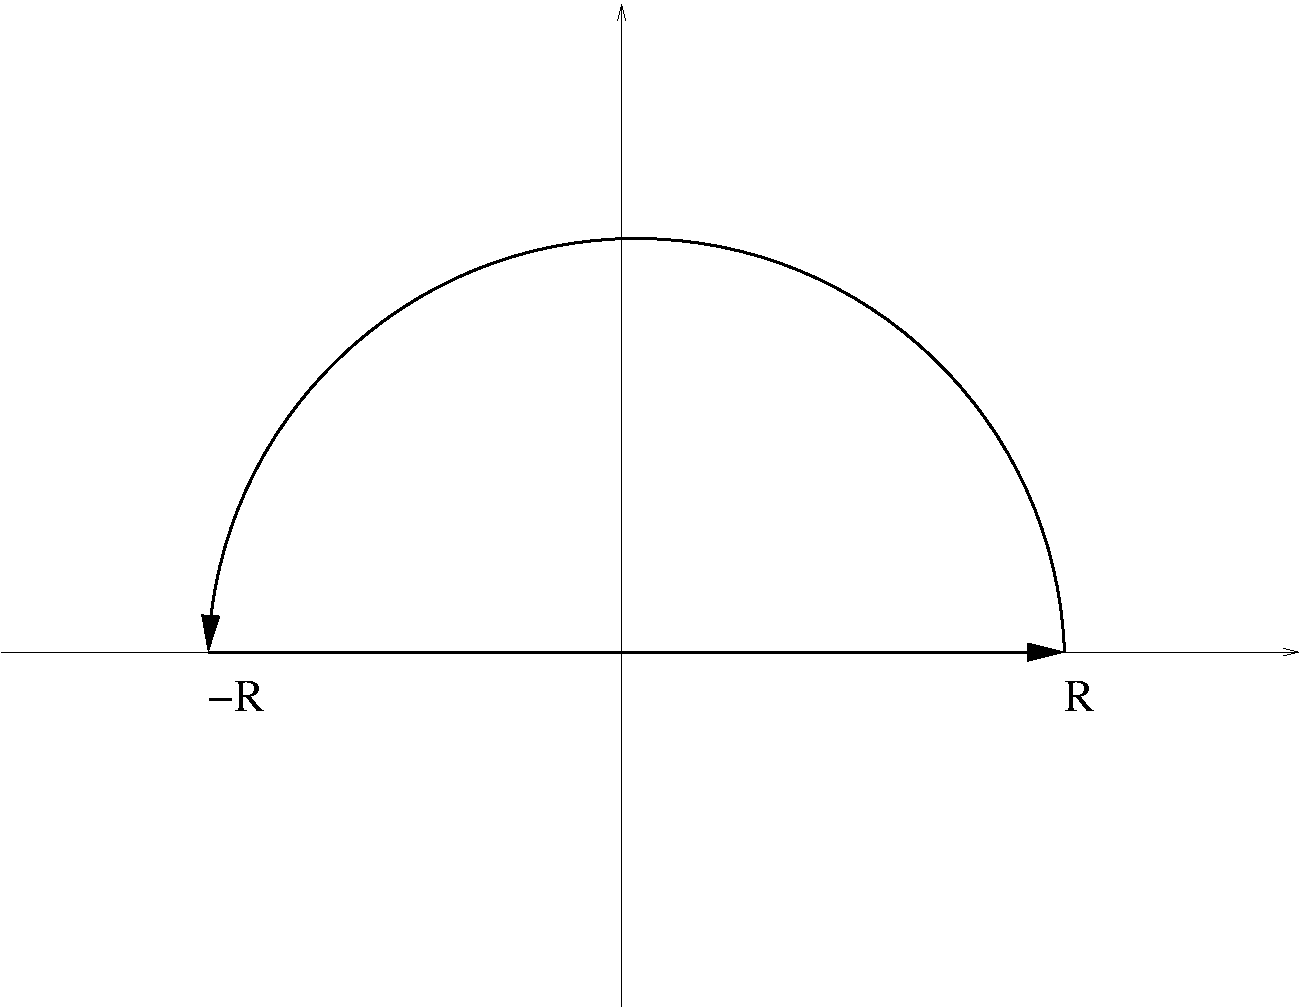
\includegraphics[scale=0.3]{images/contour_ex1.pdf}
\caption{Contour d'intégration}\label{fig:contour_ex1}
\end{figure}
\begin{enumerate}
 \item Pour $R > 1$, le point $i$ se trouve à l'intérieur du contour
d'intégration $\gamma$. On a donc:
\[
 \int_\gamma \frac{\exp(iaz)}{z+i} \frac{dz}{z-i} = i 2 \pi \frac{\exp(-a)}{2i}
= \pi \exp(-a)
\]
\item On applique le lemme de Jordan:
\[
\left|z\frac{\exp(iaz)}{z^2+1}\right| = \frac{|z|\exp(-a\Im(z))}{|1+z^2|}
\]
Sur le demi-cercle, $\Im(z) \leq 0$, d'où:
\[
\frac{|z|\exp(-a\Im(z))}{|1+z^2|} \leq \frac{R}{R^2-1}
\]
qui a pour limite 0 lorsque $R \to +\infty$.
\item On obtient immédiatement que pour $\xi > 0$, la transformée de Fourier a
pour valeur $\pi \exp(-\xi)$. Par parité, elle vaut donc sur tout $\R$,
$\pi \exp(-|\xi|)$.

\end{enumerate}

%\begin{figure}[ht]
%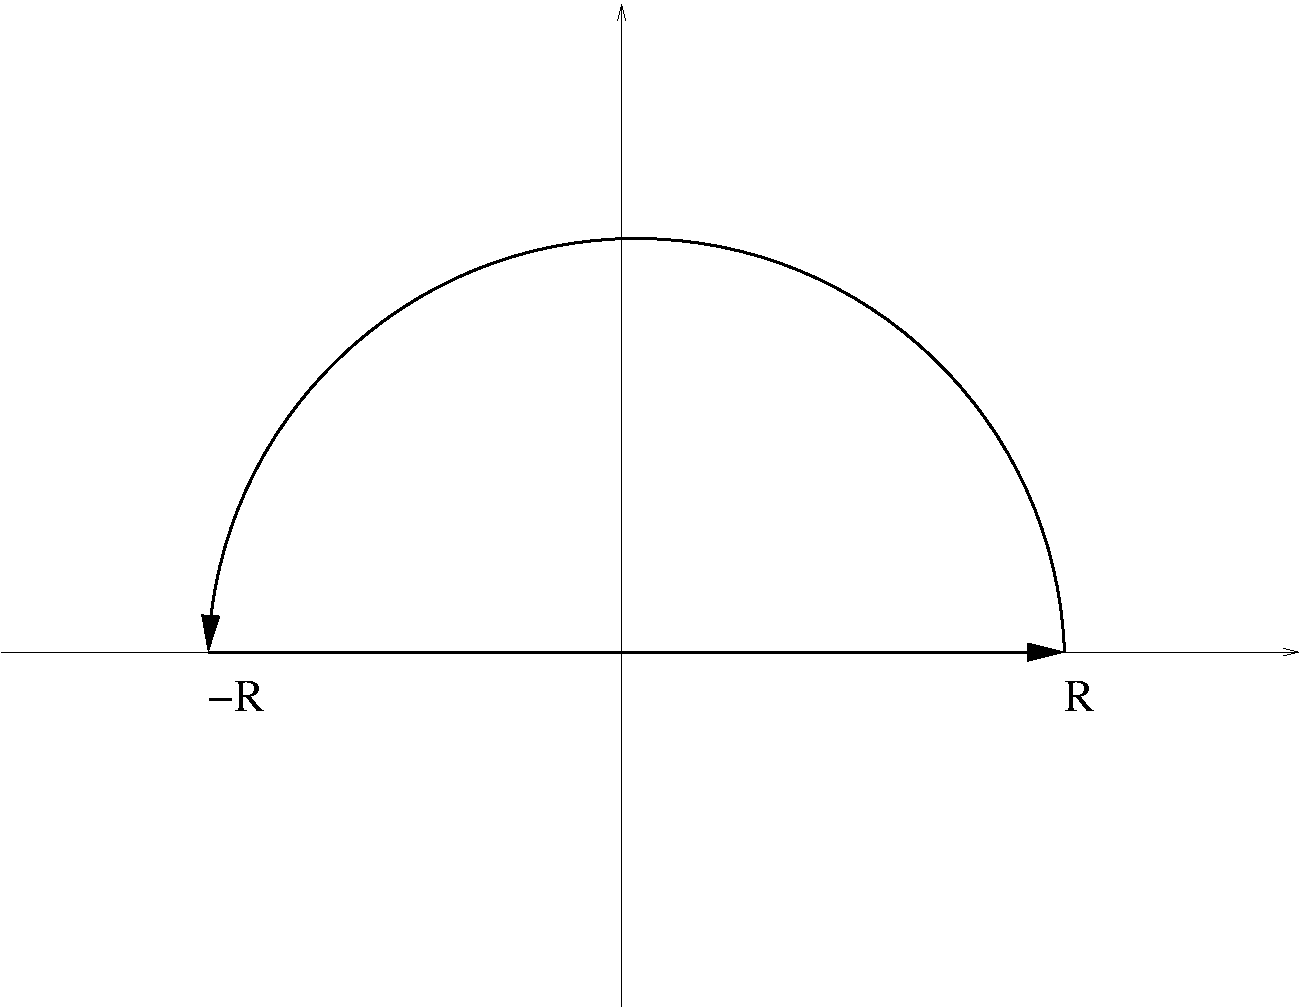
\includegraphics[scale=0.3]{images/contour_ex1.pdf}
%\caption{Contour d'intégration}\label{fig:contour_ex1}
%\end{figure}
\begin{fex}
    En utilisant la première formule de Cauchy, calculer la valeur de l'intégrale:
    \[
    \int_0^{2\pi} \frac{1}{2 + \sin x} dx
    \]
    \leftline{\textbf{Indication:}}
    Écrire le sinus sous la forme:
    \[
\sin x =\frac{e^{ix}-e^{-ix}}{2i}
    \]
    et vérifier que l'intégrale précédente est une intégrale d'une fraction rationnelle sur un lacet dans le plan
    complexe.
\end{fex} 
Quand $x$ parcourt $[0;2\pi]$ et en remplaçant $\sin$ par $e^{ix}$, on va chercher à écrire l'intégrale comme une fraction en $e^{ix}$ et intégrer sur le cercle unité. 
\begin{align*} 
    \int_0^{2\pi} \frac{1}{2 + \sin x} dx 
    &= \int_0^{2\pi} \frac{1}{2 + \frac{e^{ix}-e^{-ix}}{2i}} dx \\ 
    &= \int_0^{2\pi} \frac{2ie^{ix}}{4ie^{ix} + e^{2ix}-1} dx \\  
    &= \int_{C(0,1)} \frac{2}{4iz + z^2 - 1} dz 
\end{align*} 
Le dénominateur admet pour racines $z_1 = (-2-\sqrt{3})i$ (à l'extérieur du cercle unité) et $z_2 = (-2+\sqrt{3})i$ (à l'intérieur du cercle). 

Une application de la première formule de Cauchy donne 
\begin{align*} 
    \int_0^{2\pi} \frac{1}{2 + \sin x} dx 
    &= 2i \pi I(C(0,1), z_2) \frac{2}{z_2-z_1} \\ 
    &= \frac{2\pi}{\sqrt{3}} 
\end{align*} 
\begin{fex} 
Déterminer le développement en série de Laurent en $0$ et en $i$ de l'application:
\[
z \mapsto \frac{e^z}{z^2+1}
\]
\end{fex} 
La fonction s'écrit comme un produit de Cauchy de deux développements en série entière connus : 

En 0 : 
\begin{align*} 
    \frac{e^z}{1+z^2} &= \left( \sum_{n \geq 0} \frac{z^n}{n!} \right) \left( \sum_{n \geq 0} (-1)^n z^{2n} \right) \\ 
    &= 1 + z - \frac{z^2}{2!} - \frac{5z^3}{3!} + ... 
\end{align*} 
Le rayon de convergence de cette série vaut 1 (distance à la plus proche singularité) 

En $i$ : 
\[ 
    e^z = e^i e^{z-i} = e^i \sum_{n \geq 0} \frac{(z-i)^n}{n!} 
\] 
\[ 
    \frac{1}{1+z^2} = \frac{1}{(z-i)(z+i)} =  
    \frac{1}{(z-i)(2i+(z-i))} = \frac{1}{2i(z-i)(1+\frac{z-i}{2i})} 
\] 
Or $|z-i/(2i)| < 1 $ donc 
\[
    \frac{1}{1+\frac{z-i}{2i}} = \sum_{n \geq 0} \left( \frac{z-i}{2i} \right) ^ n 
\]
On obtient 
\begin{align*} 
    \frac{e^z}{1+z^2} 
    &= \frac{e^i}{2i} \frac{1}{z-i} \left( \sum_{n \geq 0} \frac{(z-i)^n}{n!} \right) \left( \sum_{n \geq 0} \left( \frac{1}{2i} \right) ^ n (z-i)^n \right) \\ 
    %&= 1 + z - \frac{z^2}{2!} - \frac{5z^3}{3!} + ... 
\end{align*} 

    % &= \left( \sum_{n \geq 0} \frac{z^n}{n!} \right) \left( \sum_{n \geq 0} (-1)^n z^{2n} \right) \\ 
    % &= 1 + z - \frac{z^2}{2!} - \frac{5z^3}{3!} + ... 
%\end{align*} 
\begin{fex}
 Calculer l'intégrale généralisée~:
\[
I = \int_0^{+\infty} \frac{x^2 \cos(ax)}{1+x^4} dx , \quad a \in
\mathbb{R}
\]
\end{fex} 
L'intégrale est absolument convergente~:
\[
\left |  \frac{x^2 \cos(ax)}{1+x^4} \right | \leq \frac{x^2}{1+x^4}
\]
On supposera $a\geq0$ en toute généralité puisque le cosinus est une application
paire.
Soit $f_1 : z \to \frac{z^2 e^{iaz}}{1+z^4}$ que l'on intègre sur le contour
de l'exercice précédent.
Le lemme de Jordan s'applique directement sur le demi-cercle~:
\[
\left |
\frac{z^3 e^{iaz}}{1+z^4} 
\right | \leq \frac{|z|^3 e^{-a \Im(z)}}{|1-|z|^4|}
\]
Les pôles de $f$ dans le domaine intérieur au contour sont, pour $R$ assez
grand~:
\[
z_1 = e^{i\frac{\pi}{4}}, \, z_2 = e^{i\frac{3\pi}{4}}
\]
On utilise la formule du cours pour calculer le résidu d'une fraction
rationnelle en un pôle simple~: 
\[
Res(z_k) = \frac{z_k^2 e^{ia z_k}}{4 z_k^3}
\]
On en déduit après calculs~:
\[
I = \frac{\pi e^{-a/\sqrt{2}}}{2\sqrt{2}} \left (
\cos\frac{a}{\sqrt{2}} - \sin \frac{a}{\sqrt{2}} \right )
\]

\begin{fex}
 Calculer l'intégrale généralisée~:
\[
I = \int_0^{+\infty} \frac{ \sin x}{x}dx
\]
\end{fex}
On utilise l'application $g : z \to \frac{e^{iz}}{z}$ et le contour $\gamma$ donné en
figure \ref{fig:contour_sinc}. 
$g$ est
holomorphe dans le domaine intérieur au contour on a donc:
\[
\int_{\gamma} g(z) dz = 0
\]

Par continuité
de $g$, la  limite de l'intégrale
Le demi-cercle de rayon intérieur de rayon $\epsilon$, noté $\gamma_4$, se paramètre par:
\[
t \in [0,\pi] \mapsto \epsilon e^{it}
\]
On peut évaluer l'intégrale de $g$ le long de $\gamma_4$ avec la formule vue en cours:
\[
\int_{\gamma_4}^{} g(z) dz = \int_0^\pi \frac{e^{i\epsilon(\cos t + i \sin t)}}{\epsilon e^{it}}i \epsilon e^{it}dt = i \int_0^\pi e^{i\epsilon(\cos t + i \sin t)} dt
\]
Le théorème de convergence dominée s'applique, on en déduit que la limite de cette intégrale pour $\epsilon$ tendant vers 0 est $i \pi$. Dans le contour $\gamma$, le demi-cercle est parcouru en sens inverse, on devra donc prendre $-i \pi$. 
Sur le
demi-cercle extérieur (de rayon $R$), on majore l'intégrale (voir exercice 2.6) par~:
\[
2 \int_{[0, \frac{\pi}{2}]} e^{- \frac{2 R t}{\pi}} d\lambda(t)
\]
prouvant que la limite est $0$ lorsque $R$ tend vers l'infini\footnote{on peut également utiliser la convergence dominée après un 
paramétrage du demi-cercle}.
 On obtient finalement que la valeur de
l'intégrale généralisée demandée est $\frac{\pi}{2}$.
\begin{figure}[ht]
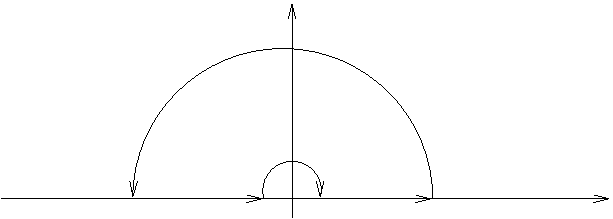
\includegraphics[scale=1]{images/contour_sinc.pdf}
\caption{Contour d'intégration}\label{fig:contour_sinc}
\end{figure} 
\begin{fex} 
    Calculer les trois premiers termes non nuls du développement en série de Laurent de $\cot z$ au voisinage de l'origine.
\end{fex} 
On a:
\[
\begin{split}
    & \sin(z) = \sum_{n\geq 0} (-1)^n \frac{z^{2n+1}}{(2n+1)!} \\
     & \cos(z) = \sum_{n\geq 0} (-1)^n \frac{z^{2n}}{(2n)!}
\end{split}
\]
En appliquant l'algorithme de division selon les puissances croissantes, il vient:
\[
\frac{\cos z}{\sin z} = \frac{1}{z} - \frac{z}{3} - \frac{z^3}{45}
\]
\begin{fex} 
On veut déterminer l'original de l'application~:
\[
F : p \to \frac{1}{1+p^3}
\]
\begin{itemize} 
\item Calculer, en précisant l'abscisse de convergence, la transformée de Laplace de l'application:
\[
f \colon t \mapsto \begin{cases}
    0 & t< 0 \\
    e^{-at} & t \geq 0, a \in \C
\end{cases}
\]
\item Décomposer $F$ en éléments simples et en déduire son original $f.$
\item Retrouver ce résultat par la formule d'inversion de Mellin-Fourier.
\end{itemize} 
\end{fex} 
Une primitive de l'application $t \mapsto e^{-(a+p)t}$ est:
\[
-\frac{e^{-(a+p)t}}{p+a}
\]
On en déduit que l'intégrale de Laplace:
\[
\int_0^{+\infty} e^{-(a+p)t} dt
\]
est convergente si et seulement si $\Re{p}> -\Re{a}.$
Elle vaut alors:
\[
\mathcal{L}(f)(p) = \frac{1}{p+a}
\]
La décomposition en éléments simples de $F$ est:
\[
\frac{1}{1+p^3} = \frac{1}{3} \frac{1}{1+p}
+\frac{e^{-i 2 \pi /3}}{3}\frac{1}{1-e^{i\pi /3}} 
+\frac{e^{i 2 \pi /3}}{3}\frac{1}{1-e^{-i \pi /3}}
\]
L'original de $F$ est donc, après simplification:
\[
\frac{1}{3} e^{-t} \left(1+\sqrt{3} e^{\frac{3 t}{2}} \sin \left(\frac{\sqrt{3} t}{2}\right) -e^{\frac{3 t}{2}} \cos \left(\frac{\sqrt{3} t}{2}\right)\right)
\]

On remarque tout d'abord que les coefficients de la décomposition en éléments simples sont les résidus de $F$ sur les trois points singuliers $-1,e^{i \pi/3},e^{-i \pi /3}.$ On intègre sur le contour \ref{fig:contour_laplace}:
\begin{figure}
    \centering
    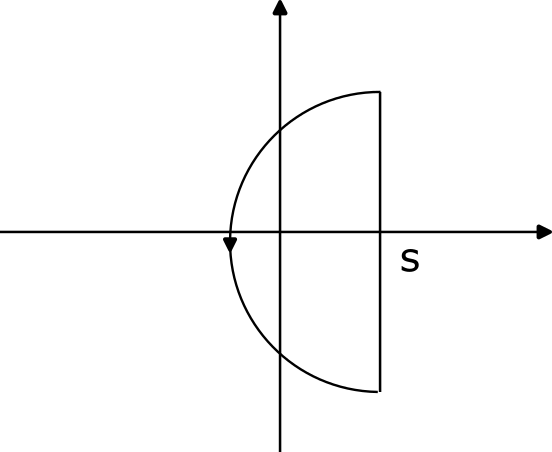
\includegraphics{images/contour_laplace.png}
    \caption{Contour pour Mellin-Fourier.}
    \label{fig:contour_laplace}
\end{figure}
avec $s > 1/2$, par exemple $s=1.$
Sur le demi-cercle de rayon $R > 2$, on majore l'intégrale par l'inégalité ML, soit:
\[
\pi \frac{R}{R^3-2} 
\]
qui admet pour limite $0$ lorsque $R$ tend vers $+\infty$.
On conclut alors par la formule d'inversion de Mellin-Fourier.
\end{document} 